\chapter{Methodology and Implementation}
\label{chap:metodology}

Our goal with this project as outlined in \cref{chap:introduction} is creating a method for identifying LN relevant transactions on the blockchain and discover what information will be available to us by doing so. The LN is a separate network but the on-chain transactions it requires for operating channels gives us a link between the two. Because we are interested in what we can learn about the LN and its users from analyzing the blockchain, we will not utilize the information in non LN relevant transactions or users in this project. Reason behind this is the size of the blockchain as discussed in \cref{sec:related}, which means the requirements for both software and hardware will be high if all information should be kept track for parsing. The benefits of taking all information into consideration are also small four our project, however, it can be helpful and is discussed further in \cref{sec:future} on future work. 
\\

The link between the LN and the Bitcoin network will only provide us with a portion of the information about the LN and its users. By connecting to the LN itself we would have access to more information than found on the blockchain. However, the LN is a dynamic changing network of nodes, channels, and payment's; which is not stored in any public ledger like the blockchain. The information found in the LN can be recorded and stored by participants but the system itself does not keep such a record. The data in the blockchain can be verified by any user as explained in \cref{subsec:blockchain} while data recorded from the LN could not be verified in the same manner on its own.
This means that if we want historical data about the LN we must use the blockchain in which the users maintain a consensus about its correctness. Because as already stated the LN requires the Bitcoin system to operate so there will be on-chain transactions on the blockchain. We can also use the fact that there is much information available from connecting to the LN itself: collecting this information will allow us compare it with what we find on the blockchain. Doing this comparison we can verify our method for identifying LN relevant transactions on the blockchain. 
In this project we have created a method for identifying LN relevant transactions while parsing the blockchain, collected data from the LN to compare to the blockchain data, and applied methods for linking relevant information to reveal non-explicit information. 
%analysis of anonymity include.

\section{Blockchain analysis}

The transactions in the blockchain is linked with outputs - inputs forming a DAG as we explained in \cref{subsec:transactions}. Parsing the blockchain would entail linking these transactions to form a transaction graph. When applying the heuristics used by previous works discussed in \cref{sec:background} one can use the information discovered there to provide context to the graph. In our work we do not create a complete transaction graph; we only link transactions related to a single LN channel which gives us a set of sub graphs of the complete transaction graph, each representing LN a channel. Only creating these small sub graphs is considerably easier because we do not need keep track as much data when the parsing is done. To create these graphs we must first differentiate between on-chain LN transactions and normal Bitcoin transactions.
\\

To locate LN relevant transaction on the blockchain we identified attributes they contained not present in other transactions. As stated in \cref{subsec:pcln} Lightning channels have two main on-chain transactions: the founding/opening and closing transaction as seen in \cref{fig:ln_tx_graph} with the two middle transactions. The founding transaction will contain the channel output, and the closing transaction will have the channel input. This output - input pair will be of the type P2WSH 2of2 mutlsig as stated in \cref{subsec:pcln}. This will be the case for all output - input pairs used for these on-chain transactions, but it is not sufficient to determine if a transaction is related to the LN or not, because P2WSH 2of2 multisig transactions can be used for other purposes. As we explained in \cref{subsec:scripts} a P2SH (non segwit version of P2WSH) lock type will only have the hash of the script in the output, while the redeem script itself is included in the input of the spending transaction. This means that if we only consider a founding transaction output we will only be able to tell if the output is a P2WSH type, but if we only look at the closing tx input we will be able to tell that the type is P2WSH and that the redeem script is a 2of2 multisig script. Since both properties must be present in a LN channel output - input pair, we can say that it is more likely the transactions containing the inputs is relevant to LN based on the closing transaction rather than the founding tx. While this method cannot determine if transactions is related to the LN or not, it allows us to say that the transactions types in question are likelier than others to be LN related. We will discuss identification using this method later in this chapter.
\\

In addition to 2of2 multisig redeem scripts there is other script types used in certain LN on-chain transactions. One of these scripts is the one used when a channel is unilaterally closed-i.e., one of the parties in the channel publishes a commitment transaction. As explained in section \cref{subsec:pcln} the one who publishes a commitment transaction has their output of the commitment timelocked; this is to enable punishment for the publisher if the commitment in question was a revoked one with outdated balance favoring the publisher more than the most recent commitment. As stated in the LN specification \cite{bolt3} this unilaterally published commitment transaction has two outputs: one P2WPKH to the party who did not publish, and one P2WSH output with a redeem script which can be spent by waiting for the timelock it contains or with a revocation key. 
This redeem script is fairly unique and to our knowledge there is no other instances such scripts are used. However, people are free to create such scripts without it having anything to do with the LN, but the specific use case of such script makes this unlikely. Because the redeem script is located in the transaction spending a P2WSH output, we need for this case locate it in the transaction spending the timelocket output from the closing/commitment transaction. We will refer to this as the timelocked transaction which is shown on the right in \cref{fig:ln_tx_graph}. We explained in \cref{subsec:segwit} that each transaction has a id which is a hash of the transaction. This is how the transaction refer to each other; the inputs of transactions contain the transaction hash and output index of the transaction they spend. By looking for transactions with the redeem script for timelocked outputs we can identify the timelocked transactions, and because it will contain a reference to the transactions is spends we now also can locate the commitment/closing tx. Looking at the input to the commitment/closing transaction we can in turn find the founding tx. Doing this again with the founding transaction will give use the transactions used for input to the founding transaction. We are interested in these transactions which are used for input in the founding transaction for linking purposes which will be explained in \cref{sec:linking}. Using this method of first identifying the timelocked tx and then following the references to previous transactions found in the inputs will allow us to create subgraphs with transactions related to a LN channel as shown in \cref{fig:ln_tx_graph}.

\begin{figure}[h]
    \centering
    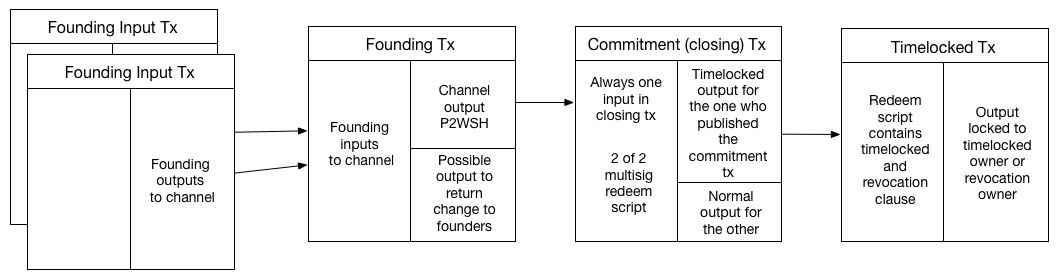
\includegraphics[width=14cm]{figures/ln_tx_graph.png}
    \caption{Transaction subgraph of unilaterally closed channel}
    \label{fig:ln_tx_graph}
\end{figure}


This method for locating subgraphs with LN related transactions is done in reverse when comparing to their creation time-i.e., we will find the timelocked transaction first and the tranactions used for input to the founding transaction last.
Because the tranasctions is a DAG as stated before, they will be located chronologically in the blockchain-e.g., the closing transactions cannot be found before the founding transaction as the closing uses the output of the founding.
We explained in \cref{subsec:blockchain} the blockchain confirms transactions and makes them valid by adding them to the chain; this means we must parse the blockchain in reverse order starting from the lastest block working our way down the the start. Doing this means we will encounter the relevant transactions in the order we want-i.e., for a subgraph we first encounter the timelocked tx and lastly the founding input transactions. We must also do this because the structure of the blockchain with blocks only referencing the previous one, only allowing us to traverse backwards in the chain. 
\\

In this project we have developed software parsing the blockchain and identified relevant transactions using the method outlined above.
We the btcd \cite{btcd_roasbeef} Bitcoin implementation for fetching and storing the blockchain data, and we also use libraries from it to read the data.
At a high level the software finds the top block from the blockchain data stored on disk and uses it as a starting point.
Then it traverses the transactions in the block and checks if they are relevant for our project, if that is the case they are stored for later use. After the transactions in a block is parsed the hash of the preceding block is used to get it from disk, and the same process is repeated.
Again, we create the LN channel transaction subgraph shown in \cref{fig:ln_tx_graph} by first looking for inputs containing the timelocked redeem script and then use the hash of the transaction that input spends to find the commitment/closing transaction.
The algorithm in its entirety is shown in \cref{fig:algo} where we the entire process of reading blocks and finding relevant transactions.
For each transaction we first check if it is a timelocked transaction, if it is we store as part of a subgraph for that channel and store the hash of the preceeding transaction (in this case the closing/commitment). As we parse tranasctions and identify tiemlocked transactions we have list of hashes known to be closing/commitment transaction, so if a transaction is not a timelocked one we check if the hash of the transaction matches any in the list. If it does we store it and finds the hash of the preceding (in this case the founding) and store it in a similar list; the same is done with founding input transactions. These hash lists are used to find all other transactions besides the timelocked in the subgraph. So for each transaction try to indeitfy it by checking if it is timelocked or the hash can be found in any of these lists. One thing to note is that a timelocked transaction can also be used as a input to a founding transaction, so we must also check found timelocked transaction against the list of founding input transactions; this will result in the same transaction being present in two subgraphs, with different role in each.

\begin{figure}[h]
    \centering
    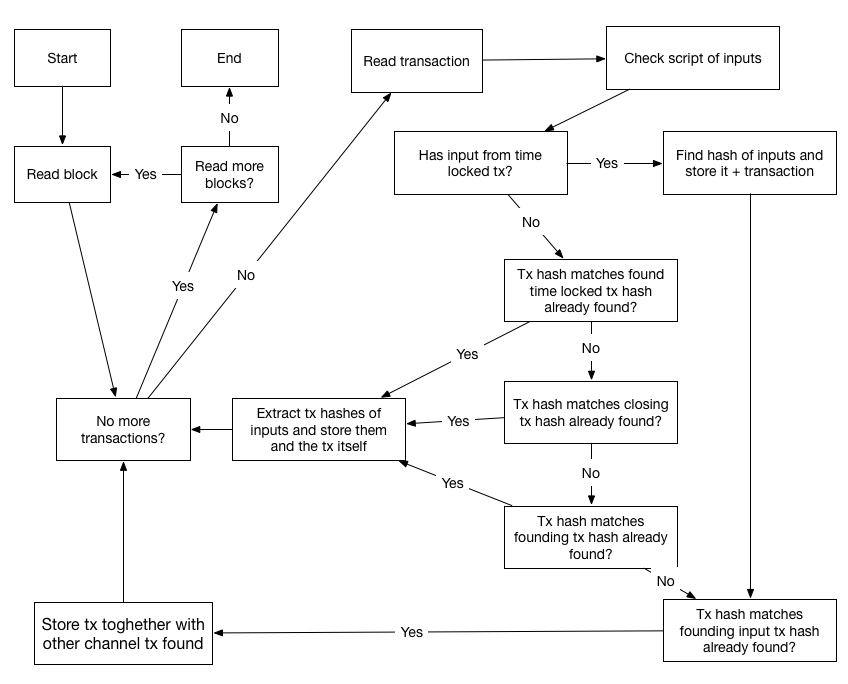
\includegraphics[width=14cm]{figures/algorithm.png}
    \caption{Algorithm of parsing and locating relevant LN transactions on the blockchain}
    \label{fig:algo}
\end{figure}


The redeem script used to identify the timelocked transactions is shown below: \cite{bolt3}
\\

\noindent OP\_IF \\
\indent   # Penalty transaction \\
\indent    <revocationpubkey> \\
OP\_ELSE\\
\indent    `to\_self\_delay`\\
\indent    OP\_CSV\\
\indent    OP\_DROP\\
\indent    <local\_delayedpubkey>\\
OP\_ENDIF\\
OP\_CHECKSIG\\

The first line is the clause to stop participants from publishing old commitment transactions. The script will evaluate to true if this clause is used and the signature for the public key is given; As discussed in \cref{subsec:pcln} the parties will revoke old commitment transactions by exchanging keys so the other party can spend the timelocked output with the revocation key and get all the founds in the channel. The else clause is the timelocked portion of the script; it will contain a delay and the CHECKSEQUENCEVERIFY operation defined in \cite{BIP112} which terminates the script if the delay has not passed. The delay is then removed from the stack with OP\_DROP such that the signature and public key are the only two items on the stack when OP\_CHECKSIG is used to very the signature.
Our implementation takes the witness stack for each transaction it checks; see \cref{subsec:segwit} where we explained how the witness stack is structured for P2WSH transactions. % example of byte encoded witness stack. detail
%check segwit mandatory.
\\

[99 33 2 126 120 157 3 221 51 166 248 112 126 125 158 170 244 190 182 208 132 33 63 68 47 200 84 246 158 249 169 162 216 193 225 103 2 177 4 178 117 33 3 123 132 176 130 116 241 4 42 10 48 64 171 85 99 123 61 247 9 119 228 167 173 206 99 118 75 52 241 193 170 236 210 104 172]
\\

Above we see the raw byte representation of the redeem script shown earlier. It contains the same operations as previously discussed as well as public keys and data. As we explained in \cref{subsec:scripts} the operations in the Bitcoin scripts is called opcodes, and the Bitcoin wiki contains a list of all of them with their encodings \cite{bitcoin_wiki_scripts}. To identify this a script of this type we use these opcodes because they will remain the same, while the public keys and delay can be variable. The first byte vector seen in the raw script above is 99 which is the opcode for the the OP\_IF operation. The next vector is 33 which indicates how many bytes to push. 33 bytes is the length of a compressed public key with prefix. Bitcoin uses elliptic curve cryptography, 
% multisig detection

% how other information gathered. output types so on.

\section{Lightning network analysis}
\label{sec:ln_analysis}

% lnd introduction

%why gather ln data (relate to background and goals)

%how ln data was gathered

To gather data from the LN we used a modified version of the LND \todo{add ref} implementation, which follows the BOLT specification \todo{add ref}. It maintains a view of the network by storing a graph containing active channels. This is continuously updated as new channels are annouched and closing transactions is found on the blockchain. It requires a Bitcoin backend running to interact with the Bitcoin network; using it to publish on-chain transactions and monitor the blockchain. New channels are discovered by annouchements within the LN while channels closing is found by looking at the blockchain and finding transactions spending the founding transactions of previously active channels. We forked and modified LND to create a copy of its database each time a new block notification was received from the Bitcoin software giving us a snapshot of the network on each new block.
\\

Each snapshot we collected contained the graph describing the network in its current state, so by comparing the graphs of different snapshorts we can see how the network evolves over time. When comparing two snapshots from two points in time we can identify closed channels by checking the old snapshot for channels not found in the new one; Similarly new channels can be found by checking the new snapshot for channels not found in the old one. This allows us to build a list of closed and opened channels during the collection timeframe, as well as the those which are open throughout. 

% details getting channels.

% comparing to blockchain data

\section{Linking}
\label{sec:linking}

% intro clusting, goals and related work

% how we cluster channels and so on.